\documentclass{article}



\usepackage{fullpage}
\usepackage{nopageno}
\usepackage{amsmath}
\usepackage{amsfonts}
\usepackage{graphicx}
\usepackage{framed}
\usepackage{xcolor}

\definecolor{dark_red}{rgb}{0.5,0.0,0.0}
\definecolor{dark_green}{rgb}{0.0,0.5,0.0}
\definecolor{dark_blue}{rgb}{0.0,0.0,0.5}

\newcommand{\dr}[1]{\textcolor{dark_red}{#1}}
\newcommand{\dg}[1]{\textcolor{dark_green}{#1}}
\newcommand{\db}[1]{\textcolor{dark_blue}{#1}}


\begin{document}

\section{Angles and parallel lines}

\begin{tabular}{cc}
\parbox{0.5\textwidth}{
In the image on the right, two parallel lines \(L_1\) and \(L_2\) are shown. Line \(M\) is not parallel to \(L_1\) and \(L_2\). Line \(M\) will intersect both \(L_1\) and \(L_2\), and the angles present at the intersections are identical. 
} & 
\parbox{0.5\textwidth}{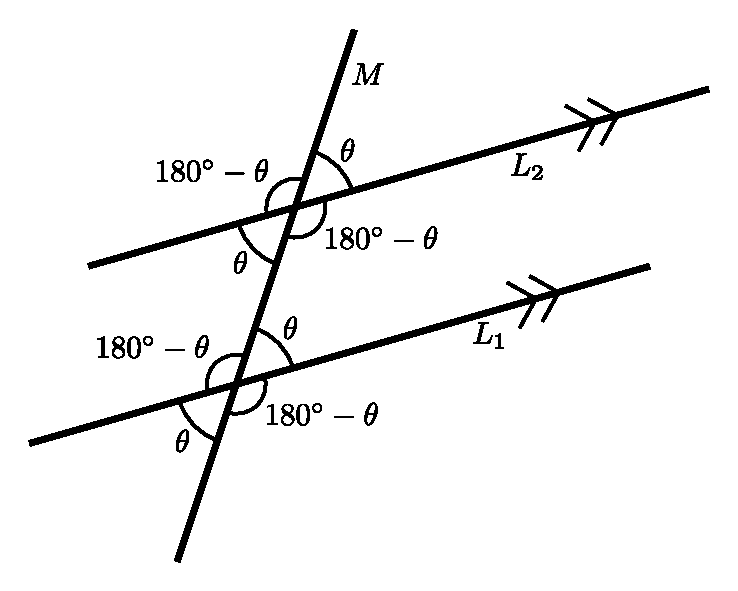
\includegraphics[width = 0.5\textwidth]{angles_and_parallel_lines}} 
\end{tabular}

\begin{tabular}{cc}
\parbox{0.5\textwidth}{
A special case of the above scenario is when the lines form the shape of the letter ``Z" (or its reflection), as shown on the right. {\bf The interior angles at the ``Z"s vertices are equal.} This  property is used extensively in computing angles from other angles, as demonstrated in the following observations/proofs.
} & 
\parbox{0.25\textwidth}{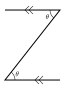
\includegraphics[width = 0.25\textwidth]{Z_angles}}
\end{tabular}

\begin{tabular}{cc}
\parbox{0.4\textwidth}{
The interior angles of any triangle sum to \(180^\circ\). The ``proof" of this is depicted in the image to the right. The dashed line that passes through the top vertex is parallel to the base. The angle that the dashed line makes with the left side of the triangle is equal to the interior angle \(\theta_A\) that the left side makes with the base. The angle that the dashed line makes with the right side of the triangle is equal to the interior angle \(\theta_B\) that the right side makes with the base. At the top vertex, angles \(\theta_A\), \(\theta_B\), and \(\theta_C\) clearly sum to \(180^\circ\).
} & 
\parbox{0.5\textwidth}{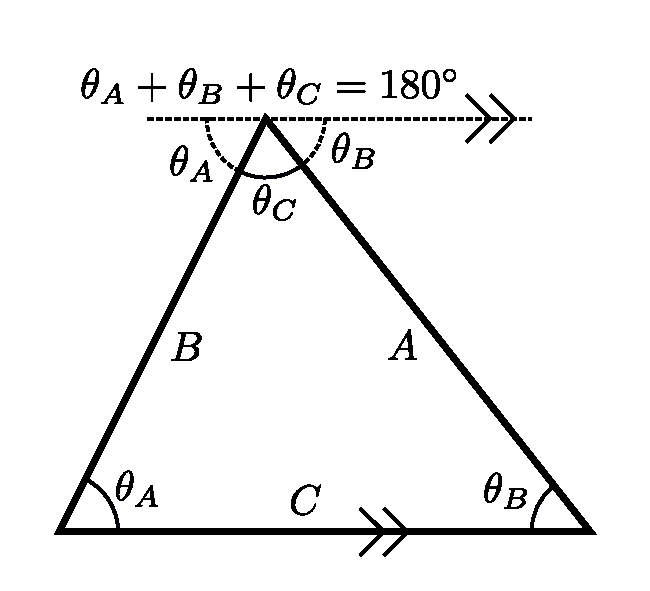
\includegraphics[width = 0.5\textwidth]{triangle_angles_sum_to_180}}
\end{tabular}

\begin{tabular}{cc}
\parbox{0.4\textwidth}{
A ``right triangle" is a triangle that has a \(90^\circ\) angle. From the fact that the interior angles of a triangle sum to \(180^\circ\), the non right angles of a right triangle sum to \(90^\circ\), as demonstrated in the image to the right. The angle that the ``hypotenuse" makes with the dashed line is equal to the angle \(\theta\) that the hypotenuse makes with the horizontal side.
} & 
\parbox{0.5\textwidth}{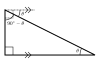
\includegraphics[width = 0.5\textwidth]{right_triangle_angles_sum_to_90}}
\end{tabular}





\section{Scaling and similarity}

Two shapes are ``similar" is they have the same proportions:

%%%%%%%% Similar triangles 1
\begin{tabular}{cc}
\parbox{0.4\textwidth}{
In the image to the right, the two triangles are ``similar", which means they have identical proportions. This is reflected in the fact that the angles of the triangles are identical, though the second triangle has also been rotated relative to the first triangle. 
To find the missing length \(A'\) in the second triangle, there are two approaches. 
} & 
\parbox{0.5\textwidth}{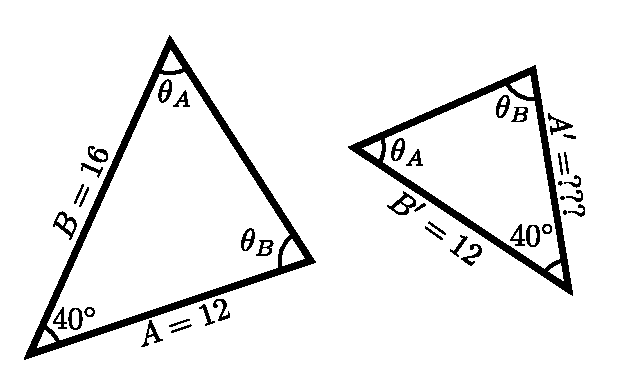
\includegraphics[width = 0.5\textwidth]{similar_triangles_1}}
\end{tabular} \\

\textbf{Approach \#1} \\
In the first (left) triangle, the number of units of side length \(A\) per unit of side length \(B\) is \(r = \frac{A}{B} = \frac{12}{16} = \frac{3}{4}\). This ratio also applies to the second (right) triangle, so the total number of units that form side length \(A'\) is \(B'\) copies of \(r\): \(A' = B' \cdot r = 12 \cdot \frac{3}{4} = 9\). Therefore: \(A' = 9\). 

\textbf{Approach \#2} \\
The number of copies of \(B\) needed to total to \(B'\) is \(r = \frac{B'}{B} = \frac{12}{16} = \frac{3}{4}\). The length \(A'\) is \(r\) copies of \(A\): \(A' = r \cdot A = \frac{3}{4} \cdot 12 = 9\). Therefore: \(A' = 9\).


%%%%%%%% Similar triangles 2
\begin{tabular}{cc}
\parbox{0.4\textwidth}{
In the image to the right, the two triangles are ``similar", which means they have identical proportions. This is reflected in the fact that the angles of the triangles are identical, though the second triangle has also been rotated relative to the first triangle. 
To find the missing length \(A'\) in the second triangle, there are two approaches. 
} & 
\parbox{0.5\textwidth}{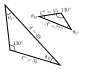
\includegraphics[width = 0.5\textwidth]{similar_triangles_2}}
\end{tabular}

\textbf{Approach \#1} \\
In the first (left) triangle, the number of units of side length \(A\) per unit of side length \(C\) is \(r = \frac{A}{C} = \frac{49}{35} = \frac{7}{5}\). This ratio also applies to the second (right) triangle, so the total number of units that form side length \(A'\) is \(C'\) copies of \(r\): \(A' = C' \cdot r = 15 \cdot \frac{7}{5} = 21\). Therefore: \(A' = 21\). 

\textbf{Approach \#2} \\
The number of copies of \(C\) needed to total to \(C'\) is \(r = \frac{C'}{C} = \frac{15}{35} = \frac{3}{7}\). The length \(A'\) is \(r\) copies of \(A\): \(A' = r \cdot A = \frac{3}{7} \cdot 49 = 21\). Therefore: \(A' = 21\).


%%%%%%%% Similar rectangles
\begin{tabular}{cc}
\parbox{0.4\textwidth}{
In the image to the right, the two rectangles are ``similar", which means they have identical proportions. 
To find the missing length \(B'\) in the larger rectangle, there are two approaches. \\
\textbf{Approach \#1} \\
In the smaller rectangle, the number of units of side length \(B\) per unit of side length \(A\) is \(r = \frac{B}{A} = \frac{8}{10} = \frac{4}{5}\). This ratio also applies to the larger rectangle, so the total number of units that form side length \(B'\) is \(A'\) copies of \(r\): \(B' = A' \cdot r = 15 \cdot \frac{4}{5} = 12\). Therefore: \(B' = 12\). 
} & 
\parbox{0.5\textwidth}{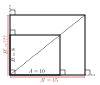
\includegraphics[width = 0.5\textwidth]{similar_rectangles}}
\end{tabular}

\textbf{Approach \#2} \\
The number of copies of \(A\) needed to total to \(A'\) is \(r = \frac{A'}{A} = \frac{15}{10} = \frac{3}{2}\). The length \(B'\) is \(r\) copies of \(B\): \(B' = r \cdot B = \frac{3}{2} \cdot 8 = 12\). Therefore: \(B' = 12\).



\section{Angular measurements}

Angles are generally measured in a counterclockwise direction. If an angle is measured in a clockwise direction, then it is negative.

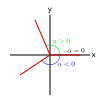
\includegraphics[width = 0.5\textwidth]{standard_angle_positions}

Angles are most commonly measured using degrees (\(^\circ\)): \(360^\circ\) for a full rotation; \(180^\circ\) for a half rotation; and \(90^\circ\) for a quarter rotation. The problem with degrees is that the choice of \(360^\circ\) for a full rotation is arbitrary an not mathematically objective. One can also make arguments in favor of \(400\) units per full rotation. {\bf Radians} will provide a mathematically objective measurement of angles.

Angles are unchanged by uniform scaling:

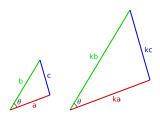
\includegraphics[width = 0.75\textwidth]{triangle_scaling}

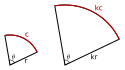
\includegraphics[width = 0.75\textwidth]{sector_scaling}

The ratio between arc length and radius depends only on the angle. This ratio, which is the angle measure in {\bf radians}, is \emph{unitless}. 

The ``unit circle" is a circle with a radius of \(1\). A sector of the unit circle with an angle of \(\theta_{\text{rad}}\) has an arc length of \(\theta_{\text{rad}}\). 

\(180^\circ = \pi \; \text{rad}\) ~~~ so ~~~ \(1^\circ = \frac{\pi}{180}\text{rad}\) ~~~ and ~~~ \(1\;\text{rad} = \frac{180^\circ}{\pi}\)

If \(\theta_{\text{deg}}\) is an angle measurement in degrees, and \(\theta_{\text{rad}}\) is a measurement of the same angle in radians, then \(\theta_{\text{rad}} = \frac{\pi}{180}\theta_{\text{deg}}\) and \(\theta_{\text{deg}} = \frac{180}{\pi}\theta_{\text{rad}}\)

\begin{tabular}{|c|c|}
\hline
Degrees & Radians \\
\hline
\hline
\(0^\circ\) & \(\frac{\pi}{180} \cdot 0 = 0\) \\
\hline
\(30^\circ\) & \(\frac{\pi}{180} \cdot 30 = \pi/6\) \\
\hline
\(45^\circ\) & \(\frac{\pi}{180} \cdot 45 = \pi/4\) \\
\hline
\(60^\circ\) & \(\frac{\pi}{180} \cdot 60 = \pi/3\) \\
\hline
\(90^\circ\) & \(\frac{\pi}{180} \cdot 90 = \pi/2\) \\
\hline
\(120^\circ\) & \(\frac{\pi}{180} \cdot 120 = 2\pi/3\) \\
\hline
\(135^\circ\) & \(\frac{\pi}{180} \cdot 135 = 3\pi/4\) \\
\hline
\(150^\circ\) & \(\frac{\pi}{180} \cdot 150 = 5\pi/6\) \\
\hline
\(180^\circ\) & \(\frac{\pi}{180} \cdot 180 = \pi\) \\
\hline
\(210^\circ\) & \(\frac{\pi}{180} \cdot 210 = 7\pi/6\) \\
\hline
\(225^\circ\) & \(\frac{\pi}{180} \cdot 225 = 5\pi/4\) \\
\hline
\(240^\circ\) & \(\frac{\pi}{180} \cdot 240 = 4\pi/3\) \\
\hline
\(270^\circ\) & \(\frac{\pi}{180} \cdot 270 = 3\pi/2\) \\
\hline
\(300^\circ\) & \(\frac{\pi}{180} \cdot 300 = 5\pi/3\) \\
\hline
\(315^\circ\) & \(\frac{\pi}{180} \cdot 315 = 7\pi/4\) \\
\hline
\(330^\circ\) & \(\frac{\pi}{180} \cdot 330 = 11\pi/6\) \\
\hline
\end{tabular}

\begin{tabular}{cc}
\parbox{0.5\textwidth}{
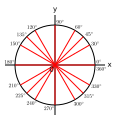
\includegraphics[width = 0.5\textwidth]{unit_circle_basic_degree_angles}
} & \parbox{0.5\textwidth}{
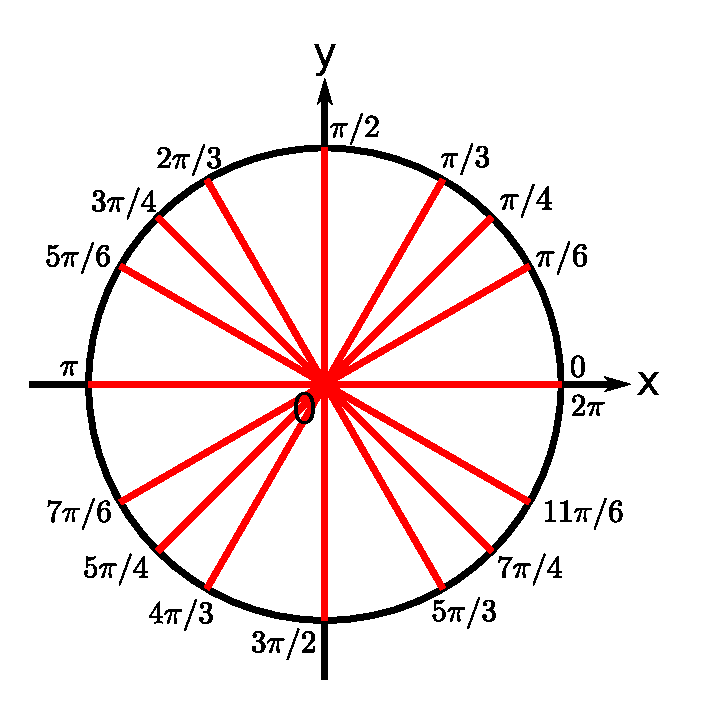
\includegraphics[width = 0.5\textwidth]{unit_circle_basic_radian_angles}
}
\end{tabular}

\textbf{Examples:}

\begin{itemize}
\item \(75^\circ = \frac{\pi\;\text{rad}}{180^\circ}(75^\circ) = \frac{75}{180}\pi\;\text{rad} = \frac{25}{60}\pi\;\text{rad} = \frac{5}{12}\pi\;\text{rad}\)
\item \(15^\circ = \frac{\pi\;\text{rad}}{180^\circ}(15^\circ) = \frac{15}{180}\pi\;\text{rad} = \frac{5}{60}\pi\;\text{rad} = \frac{1}{12}\pi\;\text{rad}\)
\item \(170^\circ = \frac{\pi\;\text{rad}}{180^\circ}(170^\circ) = \frac{170}{180}\pi\;\text{rad} = \frac{17}{18}\pi\;\text{rad}\)
\item \(200^\circ = \frac{\pi\;\text{rad}}{180^\circ}(200^\circ) = \frac{200}{180}\pi\;\text{rad} = \frac{20}{18}\pi\;\text{rad} = \frac{10}{9}\pi\;\text{rad}\)
\item \(320^\circ = \frac{\pi\;\text{rad}}{180^\circ}(320^\circ) = \frac{320}{180}\pi\;\text{rad} = \frac{32}{18}\pi\;\text{rad} = \frac{16}{9}\pi\;\text{rad}\)
\end{itemize} 

\begin{itemize}
\item \(\pi/5\;\text{rad} = \frac{180^\circ}{\pi\;\text{rad}}(\pi/5\;\text{rad}) = \frac{180^\circ}{5} = 36^\circ\)
\item \(\pi/9\;\text{rad} = \frac{180^\circ}{\pi\;\text{rad}}(\pi/9\;\text{rad}) = \frac{180^\circ}{9} = 20^\circ\)
\item \(7\pi/9\;\text{rad} = \frac{180^\circ}{\pi\;\text{rad}}(7\pi/9\;\text{rad}) = 7\frac{180^\circ}{9} = 7(20^\circ) = 140^\circ\)
\item \(13\pi/12\;\text{rad} = \frac{180^\circ}{\pi\;\text{rad}}(13\pi/12\;\text{rad}) = 13\frac{180^\circ}{12} = 13\frac{60^\circ}{4} = 13(15^\circ) = 195^\circ\)
\item \(9\pi/5\;\text{rad} = \frac{180^\circ}{\pi\;\text{rad}}(9\pi/5\;\text{rad}) = 9\frac{180^\circ}{5} = 9(36^\circ) = 324^\circ\)
\end{itemize}




\subsection{Arc-lengths and sector area}

\begin{tabular}{cc}
\parbox{0.5\textwidth}{
With \(\theta\) being measured in radians, the arc length \(c\) of a sector with a radius of \(R\) and an angle of \(\theta\) is \(c = R\theta\) by definition of the radian measure. \(\theta\) in radians is defined as the ratio \(c/R\). \\
\textbf{Examples:}
\begin{itemize}
\item If \(R = 3\) and \(\theta = 50^\circ\), then to compute the arc length \(c\), angle \(\theta\) must first be converted to radians. \(\theta = \frac{\pi\;\text{rad}}{180^\circ}(50^\circ) \approx 0.872665\;\text{rad}\). The arc length \(c\) is \(c = R\theta \approx 2.61800\)
\item If \(R = 4.7\) and \(\theta = 190^\circ\), then to compute the arc length \(c\), angle \(\theta\) must first be converted to radians. \(\theta = \frac{\pi\;\text{rad}}{180^\circ}(190^\circ) \approx 3.31613\;\text{rad}\). The arc length \(c\) is \(c = R\theta \approx 15.5858\)
\item If \(R = 2\) and \(c = 4\), then to compute the angle \(\theta\) in degrees, angle \(\theta\) in radians is the arc length per unit of radius: \(\theta = \frac{c}{R} = 2\;\text{rad}\). \(\theta\) in degrees is \(\theta = \frac{180^\circ}{\pi\;\text{rad}}(2\;\text{rad}) \approx 114.592^\circ\).
\end{itemize}
} & \parbox{0.5\textwidth}{
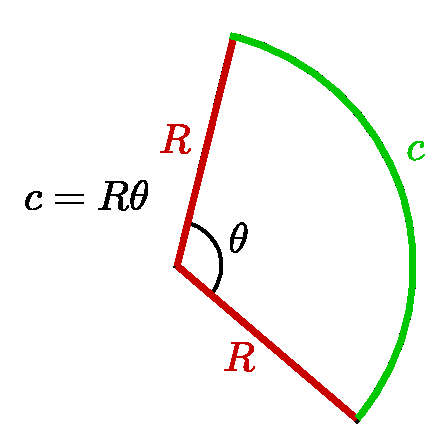
\includegraphics[width = 0.5\textwidth]{arc_length}
}
\end{tabular}
\begin{itemize}
\item If \(c = 3\) and \(\theta = 85^\circ\), then to to compute the radius \(R\), angle \(\theta\) must first be converted to radians. \(\theta = \frac{\pi\;\text{rad}}{180^\circ}(85^\circ) \approx 1.48353\;\text{rad}\). The equation \(c = R\theta\), yields \(R = \frac{c}{\theta} \approx 2.02220\)
\end{itemize}

 The sector area \(A\) is is a fraction \(\frac{\theta}{2\pi}\) of the area of the whole circle \(\pi R^2\). Hence \(A = \frac{\theta}{2\pi} \cdot \pi R^2 = \frac{1}{2}\theta R^2\)



\subsection{Coterminal angles}

Angles are {\bf coterminal} if they differ by multiples of \(360^\circ = 2\pi\;\text{rad}\). Adding or subtracting full revolutions has no effect on the angle's geometry.

\begin{itemize}
\item An angle of \(-120^\circ = -2\pi/3\) can be treated the same (is coterminal with) as \(240^\circ = 4\pi/3\) and \(-480^\circ = -8\pi/3\). 
\item An angle of \(330^\circ = 11\pi/6\) can be treated the same as \(-30^\circ = -\pi/6\) and \(690^\circ = 23\pi/6\).
\end{itemize}

To test if two angles \(\theta_1\) and \(\theta_2\) are coterminal, their difference must be an {\bf integer} multiple of \(360^\circ = 2\pi\):
\[\exists k \in \mathbb{Z} : \theta_2 - \theta_1 = k \cdot 2\pi = k \cdot 360^\circ\] 
\(k\) is the number of counter-clockwise full rotations required to reach \(\theta_2\) from \(\theta_1\).

\textbf{Examples:}

\begin{itemize}
\item Given \(\theta_1 = 3\pi/4\) and \(\theta_2 = -225^\circ\), then \(\theta_2 - \theta_1 = (-225^\circ) - 3\pi/4 = \frac{\pi}{180^\circ}(-225^\circ) - \frac{3\pi}{4}\) \(= -\frac{45\pi}{36} - \frac{3\pi}{4} = -\frac{5\pi}{4} - \frac{3\pi}{4} = -\frac{8\pi}{4} = -2\pi = (-1) \cdot 2\pi\). Since \(\theta_2 - \theta_1\) is an integer multiple of \(2\pi\), and the coefficient of \(2\pi\) is \(-1\), \(\theta_1\) and \(\theta_2\) are coterminal with \(\theta_2\) being a full clockwise revolution of \(\theta_1\).
\item Given \(\theta_1 = \pi/4\) and \(\theta_2 = -135^\circ\), then \(\theta_2 - \theta_1 = (-135^\circ) - \pi/4 = \frac{\pi}{180^\circ}(-135^\circ) - \frac{\pi}{4}\) \(= - \frac{27\pi}{36} - \frac{\pi}{4} = -\frac{3\pi}{4} - \frac{\pi}{4} = -\frac{4\pi}{4} = -\pi = (-\frac{1}{2}) \cdot 2\pi\). Since \(\theta_2 - \theta_1\) is {\bf not} an integer multiple of \(2\pi\), \(\theta_1\) and \(\theta_2\) are {\bf not} coterminal. 
\end{itemize}





\subsection{Angular and Linear speed}

Angular speed/frequency \(\omega\) is the rate of change in an angle with respect to time. Frequency \(\nu\) is the number of full revolutions per unit time. 
\[\omega = \frac{\text{angle in radians}}{\text{time}} = \frac{2\pi \times \text{number of full cycles}}{\text{time}} =  2\pi \cdot \nu\]

\begin{tabular}{cc}
\parbox{0.5\textwidth}{
In the image on the right, a gear of radius \(R\) is rotating counterclockwise at an angular speed of \(\omega\). After a time interval of \(\Delta t\), the gear has turned by \(\omega \Delta t\). The rim of the gear is moving at a speed of \(v\). After the same time interval of \(\Delta t\), the rim of the gear has moved a distance of \(v\Delta t\). The distance that the gear rim has moved can also be computed from the rotated angle of \(\omega \Delta t\) and the gear's radius \(R\): \(R \cdot \omega \Delta t\). This gives the relationship \(v \Delta t = R \omega \Delta t\) which is equivalent to:
\[v = R \omega\]
} & \parbox{0.5\textwidth}{
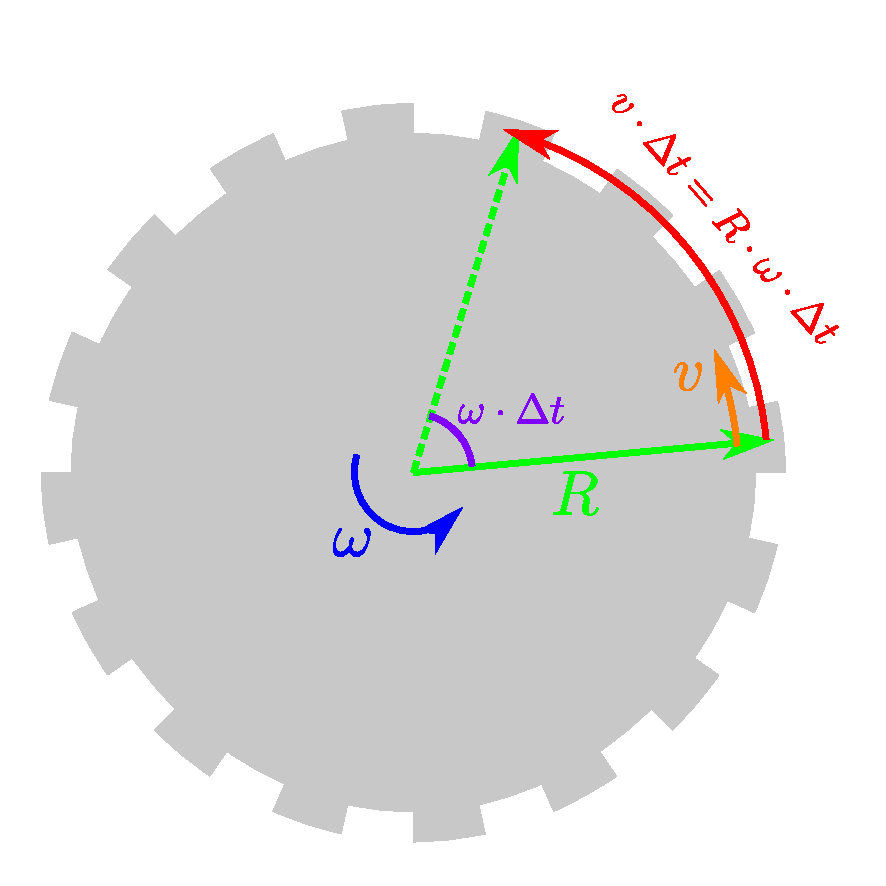
\includegraphics[width = 0.5\textwidth]{spinning_gear}
}
\end{tabular}




The linear speed (speed at the circumference) is \(v = r\omega\) \\ {\bf \(\omega\) must be measured in radians}

\textbf{Examples:}

\begin{itemize}
\item The angular speed of the Earth's rotation is \(\omega = \frac{2\pi \; \text{rad}}{(1\;\text{day})(24\;\text{h/day})(60\;\text{min/h})(60\;\text{s/min})} \approx 7.27221 \times 10^{-5} \text{rad/s}\) \\
The Earth's equatorial radius is \(R = 6378.1\text{km} = 6.37810 \times 10^6 \text{m}\) \\
The linear speed at the equator is \(v = R\omega \approx 4.63829 \times 10^2 \text{m/s} = 463.829\text{m/s}\)
%%%%%%%%%%%%
\item Angular speed of the Earth's orbit \(\omega = \frac{2\pi \; \text{rad}}{(1\;\text{year})(365.25\;\text{day/year})(24\;\text{h/day})(60\;\text{min/h})(60\;\text{s/min})} \approx \) \\ 
\(1.99102 \times 10^{-7} \text{rad/s}\) \\
The average radius of the Earth's orbit is \(R \approx 1.49598 \times 10^8\text{km} = 1.49598 \times 10^{11}\text{m}\) \\
The linear speed of the Earth in orbit around the Sun is \(v = R\omega \approx 2.97853 \times 10^4\text{m/s} = 29.7853\text{km/s}\)
%%%%%%%%%%%%
\item The international space station (ISS) orbits the earth once every \(T = 92.68\text{min} = 5.56080 \times 10^3\text{s}\) at an average altitude of \(h = 418.500\text{km} = 4.18500 \times 10^5\text{m}\) \\
The angular speed of the ISS's orbit is \(\omega  = \frac{2\pi}{T} \approx 1.12991 \times 10^{-3} \text{rad/s}\) \\
The radius of the ISS's orbit is \(R = 6.37810 \times 10^6 \text{m} + h = 6.79660 \times 10^6 \text{m}\) \\
The linear (orbital) speed of the ISS is \(v = R\omega \approx 7.67955 \times 10^3\text{m/s} = 7.67955 \text{km/s}\)
%%%%%%%%%%%%
\item If a gear has a radius of \(R = 7\text{cm} = 0.07\text{m}\), and rotates once every \(T = 2\text{s}\), then with a full rotation of \(2\pi\) every time interval of \(T\), the angular speed is \(\omega = \frac{2\pi}{T} \approx 3.14159 \text{s}^{-1}\). The speed of the rim is \(v = R\omega = 0.219911\text{m/s} = 21.9911\text{cm/s}\). \\
Reasoning in the other direction, if the rim speed is now \(v = 30\text{cm/s} = 0.300000 \text{m/s}\) and the radius is unchanged, then the angular speed satisfies \(v = R\omega \iff \omega = \frac{v}{R} \approx 4.28571 \text{s}^{-1}\). The time \(T\) required for a full revolution is: \(T = \frac{2\pi}{\omega} \approx 1.46608 \text{s}\)
\end{itemize}




\subsection{Minutes and Seconds}

In some instances, fractional degrees are quantified not by decimals, but by ``minutes" and ``seconds". Minutes and seconds in this context, are not units of time, but of angle. While degrees are denoted by the symbol \(^\circ\), minutes are are denoted by the symbol \('\), and seconds are denoted by the symbol \(''\). In a similar fashion to the units of time, there are \(60\) minutes to \(1\) degree, and \(60\) seconds to \(1\) minute:
\[60' = 1^\circ \quad \text{and} \quad 60'' = 1'\]

If a {\bf non-negative} angle (for negative angles, the \(-\) sign is factored out) is comprised of \(x\) degrees, \(y\) minutes, and \(z\) seconds, then it is denoted by \(x^\circ y' z''\) which is short for \(x^\circ + y' + z''\). Since minutes are expected to denote fractions of degrees, and seconds are expected to denote fractions of minutes, \(x\) is a non-negative integer (i.e. a whole number); \(y\) is an integer between \(0\) and \(59\) inclusive; and \(z\) is a real number that is from the interval \([0, 60)\). 

\textbf{Examples:}
\begin{itemize}
\item To convert the angle \(35^\circ4'52''\) to decimal degrees, each minute is replaced with \((1/60)^\circ\), and each second is replaced with \((1/3600)^\circ\).
\[35^\circ4'52'' = (35 + \frac{4}{60} + \frac{52}{3600})^\circ\approx 35.08^\circ\]
%%
\item To covert the angle to \(15.73^\circ\) to be use minutes and seconds, each factional component is converted to smaller units of angle.
\[15.73^\circ = 15^\circ + 0.73(60') = 15^\circ + 43.8' = 15^\circ43' + 0.8(60'') = 15^\circ43' + 48'' = 15^\circ43'48''\]
%%
\item Adding two angles involves adding the respective numbers of degrees, minutes, and seconds. Then groups of \(60''\) are converted to \(1'\) until the number of seconds is in the range \([0,60)\). Then groups of \(60'\) are converted to \(1^\circ\) until the number of minutes is an integer between \(0\) and \(59\) inclusive. 
\[6^\circ50'40'' + 7^\circ30'30'' = 13^\circ80'70'' = 13^\circ81'10'' = 14^\circ21'10''\]
\end{itemize}



\section{Right Triangle Trigonometry}

\subsection{The Pythagorean Theorem}

\begin{tabular}{cc}
\parbox{0.3\textwidth}{
In the image to the right, similar triangles are used to demonstrate the Pythagorean theorem. Given a right triangle with sides \(a\), \(b\), and \(c\) where the right angle is between sides \(a\) and \(b\), then the length of the hypotenuse \(c\) is related to \(a\) and \(b\) via \(c^2 = a^2 + b^2\). This enables one to compute \(c = \sqrt{a^2 + b^2}\); \(a = \sqrt{c^2 - b^2}\); or \(b = \sqrt{c^2 - a^2}\)
} & \parbox{0.5\textwidth}{
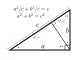
\includegraphics[width = 0.5\textwidth]{Pythagorean_Theorem}
}
\end{tabular}



\subsection{The Trigonometric Functions}

\begin{tabular}{cc}
\parbox{0.5\textwidth}{
\begin{itemize}
\item \dr{\(\cos\theta = a/h\)} is the units of adjacent per unit of hypotenuse
\item \dr{\(\sin\theta = o/h\)} is the units of opposite per unit of hypotenuse
\item \dg{\(\tan\theta = o/a = \frac{\sin\theta}{\cos\theta}\)} is the units of opposite per unit of adjacent
\item \dg{\(\sec\theta = h/a = \frac{1}{\cos\theta}\)} is the units of hypotenuse per unit of adjacent
\item \db{\(\cot\theta = a/o = \frac{\cos\theta}{\sin\theta} = \frac{1}{\tan\theta}\)} is the units of adjacent per unit of opposite
\item \db{\(\csc\theta = h/o = \frac{1}{\sin\theta}\)} is the units of hypotenuse per unit of opposite
\end{itemize}
} & \parbox{0.5\textwidth}{
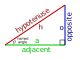
\includegraphics[width = 0.5\textwidth]{sides_of_a_right_triangle}
}
\end{tabular}

\begin{itemize}
\item If the hypotenuse \(h\) is known, then the adjacent and opposite are respectively \(\dr{a = h\cos\theta}\) and \(\dr{o = h\sin\theta}\).
\item If the adjacent \(a\) is known, then the opposite and hypotenuse are respectively \(\dg{o = a\tan\theta}\) and \(\dg{h = a\sec\theta}\).
\item If the opposite \(o\) is known, then the adjacent and hypotenuse are respectively \(\db{a = o\cot\theta}\) and \(\db{h = o\csc\theta}\).
\end{itemize}

\begin{tabular}{ccc}
\parbox{0.3\textwidth}{
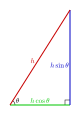
\includegraphics[width = 0.3\textwidth]{right_triangle_h}
} & \parbox{0.3\textwidth}{
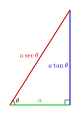
\includegraphics[width = 0.3\textwidth]{right_triangle_a}
} & \parbox{0.3\textwidth}{
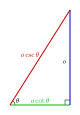
\includegraphics[width = 0.3\textwidth]{right_triangle_o}
}
\end{tabular}

\textbf{Examples:}
\begin{itemize}
\item \(h = 5\) and \(\theta = 70^\circ\) implies that \(a = 5\cos(70^\circ) \approx 1.71010\) and \(o = 5\sin(70^\circ) \approx 4.69846\) 
\item \(a = 0.5\) and \(\theta = 85^\circ\) implies that \(o = 0.5\tan(85^\circ) \approx 5.71503\) and \(h = 0.5\sec(85^\circ) \approx 5.73686\)
\item \(o = 1\) and \(\theta = \pi/4\) implies that \(a = 1\cot(\pi/4) = 1\) and \(h = 1\csc(\pi/4) \approx 1.41421\)
\end{itemize}

\begin{tabular}{cc}
\parbox{0.6\textwidth}{
Given a wall of unknown height \(h\), height \(h\) can be determined by standing a distance \(d\) from the wall and measuring the elevation \(\theta\) of the wall's summit as being viewed from the ground. The adjacent \(d\) is known and the opposite \(h\) is sought, so \(h = d \cdot \tan\theta\). \\
If \(d = 5.6\text{m}\) and \(\theta = 80^\circ\), then the wall's height is \(h = (5.6\text{m})\tan(80^\circ) \approx 31.7592\text{m}\)
} & \parbox{0.3\textwidth}{
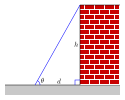
\includegraphics[width = 0.3\textwidth]{wall_height}
}
\end{tabular}

\begin{tabular}{cc}
\parbox{0.5\textwidth}{
Given a mountain with height \(h\), unlike the vertical wall from the previous example, the distance to a ground level point directly beneath the summit cannot be measured directly, as the ground level point beneath the summit is often physically inaccessible within the bulk of the mountain. To measure the mountain's height, two vantage points separated by a known distance of \(d\) are chosen where the second vantage point is directly in between the first vantage point and the ground level point beneath the summit. \(\theta_1\) and \(\theta_2\) are the line of sight elevations of the summit from the first and second vantage points respectively. {\bf Only \(d\), \(\theta_1\), and \(\theta_2\) are measured and known ahead of any computations}. 
} & \parbox{0.5\textwidth}{
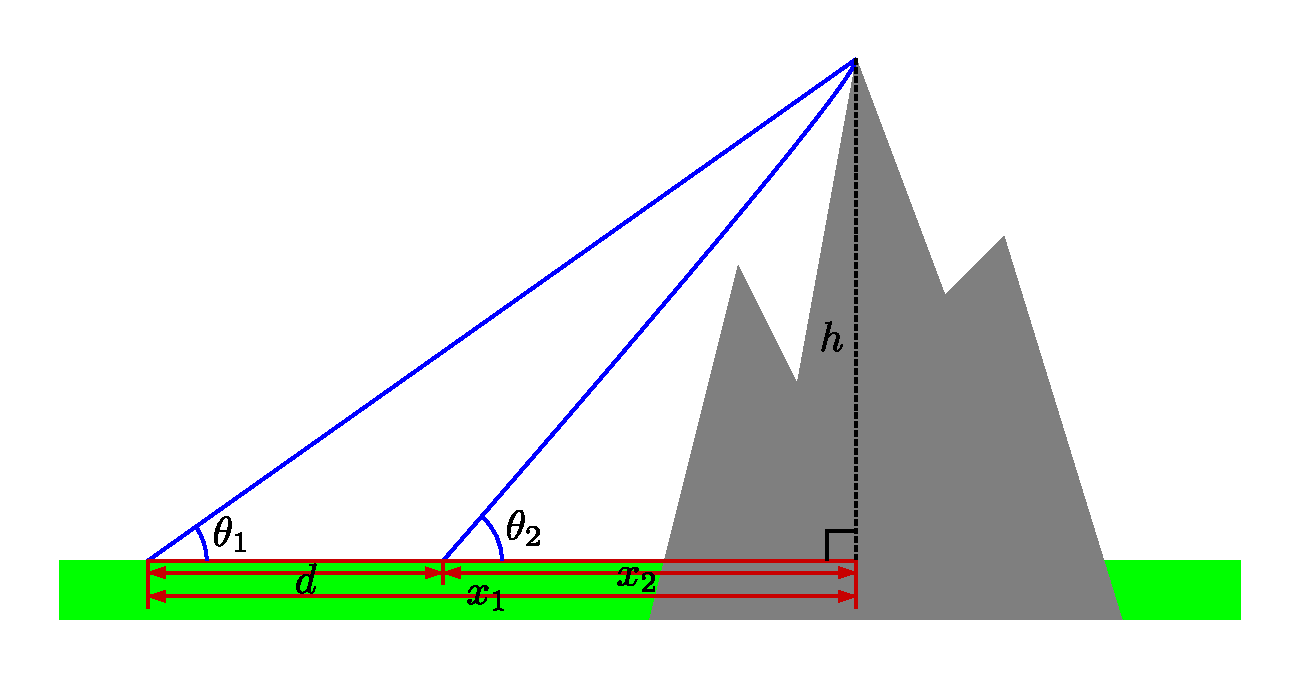
\includegraphics[width = 0.5\textwidth]{mountain_height}
}
\end{tabular}
\(x_1\) and \(x_2\) are the horizontal distances from mountain summit of the first and second vantage points respectively. The two right triangles have opposites of \(h\) and adjacents of \(x_1\) and \(x_2\)  respectively, so \(x_1 = h\cot\theta_1\) and \(x_2 = h\cot\theta_2\). \(d = x_1 - x_2\) so 
\[d = h\cot\theta_1 - h\cot\theta_2 \iff (\cot\theta_1 - \cot\theta_2)h = d \iff h = \frac{d}{\cot\theta_1 - \cot\theta_2}\]
Therefore \(h = \frac{d}{\cot\theta_1 - \cot\theta_2}\) computes the mountain's height given the ground level, accessible, measurements of \(d\), \(\theta_1\), and \(\theta_2\). As an example, given \(d = 96.0210\text{m}\), \(\theta_1 = 70^\circ\), and \(\theta_2 = 75^\circ\), then \(h = \frac{96.0210\text{m}}{\cot(70^\circ) - \cot(75^\circ)} \approx 1.00000 \times 10^3\text{m} = 1.00000\text{km}\).




\subsection{Computing sec, cot, and csc}

The trigonometric functions of \(\dg{\sec\theta}\), \(\db{\cot\theta}\), and \(\db{\csc\theta}\) do not appear on most calculators. To compute these functions, the following substitutions must be made:

\begin{itemize}
\item \(\dg{\sec\theta} = \frac{1}{\dr{\cos\theta}}\)
\item \(\db{\cot\theta} = \frac{1}{\dg{\tan\theta}}\)
\item \(\db{\csc\theta} = \frac{1}{\dr{\sin\theta}}\)
\end{itemize}




\section{The trigonometric functions of special angles}

\begin{tabular}{cc}
\parbox{0.3\textwidth}{
For \(\theta = 30^\circ = \pi/6\;\text{rad}\)
\begin{itemize}
\item \dr{\(\cos(30^\circ) = a/h = \sqrt{3}/2\)}
\item \dr{\(\sin(30^\circ) = o/h = 1/2\)}
\item \dg{\(\tan(30^\circ) = o/a = 1/\sqrt{3}\)}
\item \dg{\(\sec(30^\circ) = h/a = 2/\sqrt{3}\)}
\item \db{\(\cot(30^\circ) = a/o = \sqrt{3}\)}
\item \db{\(\csc(30^\circ) = h/o = 2\)}
\end{itemize}
For \(\theta = 60^\circ = \pi/3\;\text{rad}\)
\begin{itemize}
\item \dr{\(\cos(60^\circ) = a/h = 1/2\)}
\item \dr{\(\sin(60^\circ) = o/h = \sqrt{3}/2\)}
\item \dg{\(\tan(60^\circ) = o/a = \sqrt{3}\)}
\item \dg{\(\sec(60^\circ) = h/a = 2\)}
\item \db{\(\cot(60^\circ) = a/o = 1/\sqrt{3}\)}
\item \db{\(\csc(60^\circ) = h/o = 2/\sqrt{3}\)}
\end{itemize}
} & \parbox{0.5\textwidth}{
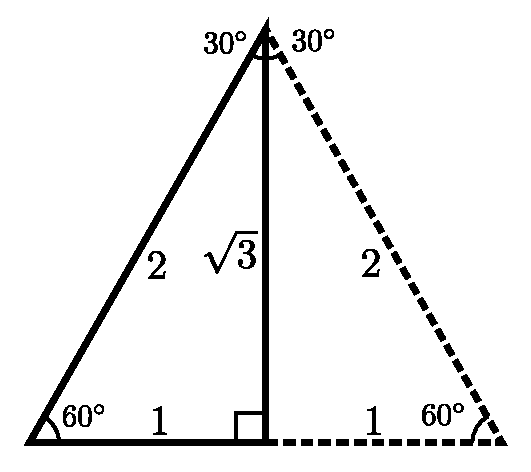
\includegraphics[width = 0.5\textwidth]{30_60_90_triangle}
}
\end{tabular}

\begin{tabular}{cc}
\parbox{0.3\textwidth}{
For \(\theta = 45^\circ = \pi/4\;\text{rad}\)
\begin{itemize}
\item \dr{\(\cos(45^\circ) = a/h = 1/\sqrt{2}\)}
\item \dr{\(\sin(45^\circ) = o/h = 1/\sqrt{2}\)}
\item \dg{\(\tan(45^\circ) = o/a = 1\)}
\item \dg{\(\sec(45^\circ) = h/a = \sqrt{2}\)}
\item \db{\(\cot(45^\circ) = a/o = 1\)}
\item \db{\(\csc(45^\circ) = h/o = \sqrt{2}\)}
\end{itemize}
} & \parbox{0.4\textwidth}{
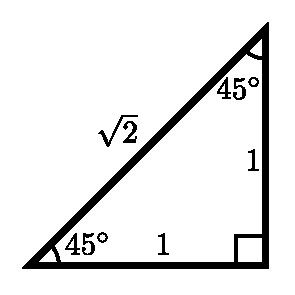
\includegraphics[width = 0.4\textwidth]{45_45_90_triangle}
}
\end{tabular}

\begin{tabular}{cc}
\parbox{0.3\textwidth}{
For \(\theta = 0^\circ = 0\;\text{rad}\)
\begin{itemize}
\item \dr{\(\cos(0^\circ) = a/h = 1\)}
\item \dr{\(\sin(0^\circ) = o/h = 0\)}
\item \dg{\(\tan(0^\circ) = o/a = 0\)}
\item \dg{\(\sec(0^\circ) = h/a = 1\)}
\item \db{\(\cot(0^\circ) = a/o = \infty\)}
\item \db{\(\csc(0^\circ) = h/o = \infty\)}
\end{itemize}
For \(\theta = 90^\circ = \pi/2\;\text{rad}\)
\begin{itemize}
\item \dr{\(\cos(90^\circ) = a/h = 0\)}
\item \dr{\(\sin(90^\circ) = o/h = 1\)}
\item \dg{\(\tan(90^\circ) = o/a = \infty\)}
\item \dg{\(\sec(90^\circ) = h/a = \infty\)}
\item \db{\(\cot(90^\circ) = a/o = 0\)}
\item \db{\(\csc(90^\circ) = h/o = 1\)}
\end{itemize}
} & \parbox{0.5\textwidth}{
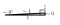
\includegraphics[width = 0.5\textwidth]{00_90_90_triangle}
}
\end{tabular}

\begin{tabular}{|c||c|c||c|c||c|c|}
\hline
\(\theta\) & \(\cos(\theta)\) & \(\sin(\theta)\) & \(\tan(\theta)\) & \(\sec(\theta)\) & \(\cot(\theta)\) & \(\csc(\theta)\) \\
\hline
\hline
\(0^\circ = 0\;\text{rad}\) & \(1\) & \(0\) & \(0\) & \(1\) & \(\infty\) & \(\infty\) \\
\hline
\(30^\circ = \pi/6\;\text{rad}\) & \(\sqrt{3}/2\) & \(1/2\) & \(1/\sqrt{3}\) & \(2/\sqrt{3}\) & \(\sqrt{3}\) & \(2\) \\
\hline
\(45^\circ = \pi/4\;\text{rad}\) & \(1/\sqrt{2}\) & \(1/\sqrt{2}\) & \(1\) & \(\sqrt{2}\) & \(1\) & \(\sqrt{2}\) \\
\hline
\(60^\circ = \pi/3\;\text{rad}\) & \(1/2\) & \(\sqrt{3}/2\) & \(\sqrt{3}\) & \(2\) & \(1/\sqrt{3}\) & \(2/\sqrt{3}\) \\
\hline
\(90^\circ = \pi/2\;\text{rad}\) & \(0\) & \(1\) & \(\infty\) & \(\infty\) & \(0\) & \(1\) \\
\hline
\end{tabular}




%\pagebreak

\section{The trigonometric functions of all angles}

The \(\dr{\cos\theta}\) and \(\dr{\sin\theta}\) where defined as the adjacent and opposite respectively when the hypotenuse is \(1\). The \(\dg{\tan\theta}\) and \(\dg{\sec\theta}\) where defined as the opposite and hypotenuse respectively when the adjacent is \(1\). The \(\db{\cot\theta}\) and \(\db{\csc\theta}\) where defined as the adjacent and hypotenuse when the opposite is \(1\). For angles outside of the range \([0, 90^\circ]\), a more general definition will be given. For acute angles, this definition will match the original definition. 

This general definition will use the \(xy\) coordinate plane. The circle that is centered on the origin with a radius of \(1\) is referred to as the ``unit circle", and is the red circle in the following diagrams. The vertical line consisting of all points where \(x = 1\) will be referred to as the ``tangent" (a tangent is a line that touches a circle at a single point, but does not enter the circle). This is the green line in the following diagrams. The horizontal line consisting of all points where \(y = 1\) will be referred to as the ``co-tangent". This is the blue line in the following diagrams. Start with a ray that is coincident with the \(x\) axis. This ray has an orientation in the positive direction of the \(x\)-axis. Given an arbitrary angle \(\theta\), rotate the ray counterclockwise an angle of \(\theta\) (if \(\theta\) is negative, the rotation is clockwise). The ray has a forwards direction, and a backwards direction. The Cartesian coordinates of the point where the \emph{forwards} ray intersects the unit circle are \(\dr{(\cos\theta, \sin\theta)}\). This is also the point arrived at by moving forwards along the ray by \(1\) unit. The Cartesian coordinates of the point where the ray, forwards or backwards, intersects the tangent are \(\dg{(1, \tan\theta)}\). The distance, which is negative if backwards, required to reach the intersection with the tangent is \(\dg{\sec\theta}\). The Cartesian coordinates of the point where the ray, forwards or backwards, intersects the co-tangent are \(\db{(\cot\theta,1)}\). The distance, which is negative if backwards, required to reach the intersection with the co-tangent is \(\db{\csc\theta}\).

In the following diagram, the unit circle is shown in red, the tangent is shown in green, and the co-tangent is shown in blue. The ray and the three intersection points are shown for an example \(\theta\) in the range \((0, 90^\circ)\) (top left image); \((90^\circ, 180^\circ)\) (top right image); \((180^\circ, 270^\circ)\) (bottom left image); and \((270^\circ, 360^\circ)\) (bottom right image).  

To better understand the connection between the definitions, the dashed gray lines trace out 3 right triangles in each diagram. With regards to the intersection point, the \(x\) coordinate is the adjacent, the \(y\) coordinate is the opposite, and the distance (which can be positive or negative) along the ray is the hypotenuse.

\begin{tabular}{cc}
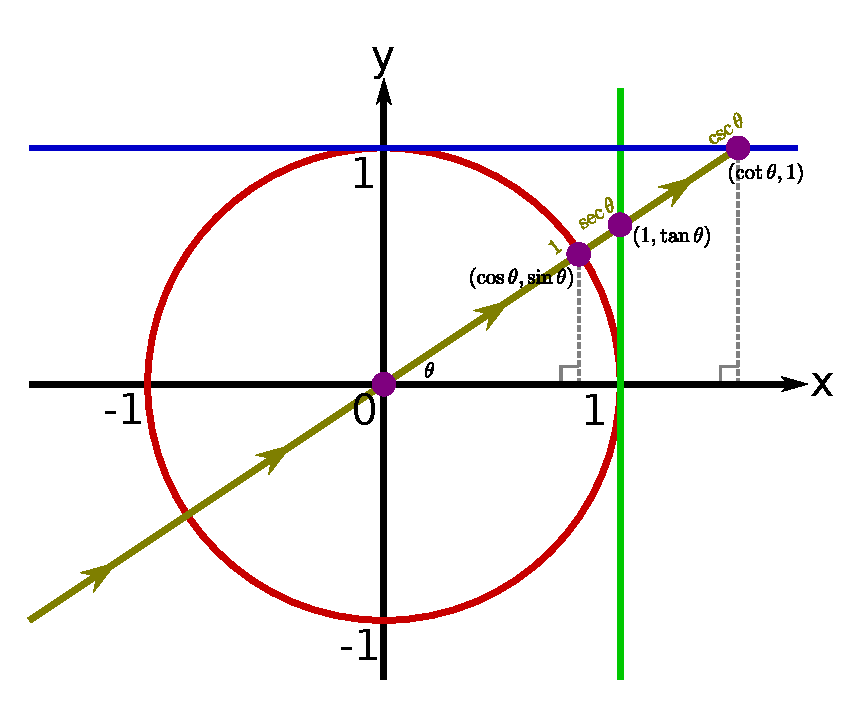
\includegraphics[scale = 0.6]{unit_circle_trig_functions_acute_angle} & 
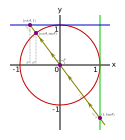
\includegraphics[scale = 0.6]{unit_circle_trig_functions_obtuse_angle} \\
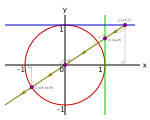
\includegraphics[scale = 0.6]{unit_circle_trig_functions_reflex_angle_1} & 
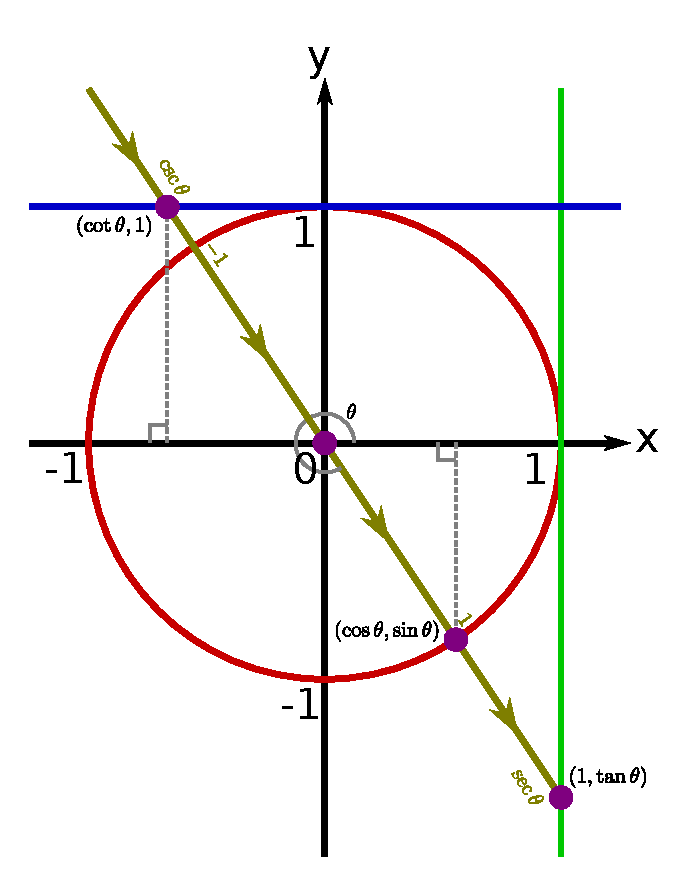
\includegraphics[scale = 0.6]{unit_circle_trig_functions_reflex_angle_2} \\
\end{tabular}

\begin{tabular}{|c||c|c||c|c||c|c|}
\hline
\(\theta\)                                           & \(\cos(\theta)\) & \(\sin(\theta)\) & \(\tan(\theta)\) & \(\sec(\theta)\) & \(\cot(\theta)\) & \(\csc(\theta)\) \\
\hline
\hline
\(0^\circ = 0\;\text{rad}\)               & \(1\)                  & \(0\)                    & \(0\)                  & \(1\)                & \(\pm\infty\)     & \(\pm\infty\)  \\
\hline
\(30^\circ = \pi/6\;\text{rad}\)        & \(\sqrt{3}/2\)    & \(1/2\)                & \(1/\sqrt{3}\)    & \(2/\sqrt{3}\)  & \(\sqrt{3}\)      & \(2\)              \\
\hline 
\(45^\circ = \pi/4\;\text{rad}\)        & \(1/\sqrt{2}\)    & \(1/\sqrt{2}\)     & \(1\)                  & \(\sqrt{2}\)      & \(1\)                & \(\sqrt{2}\)    \\
\hline
\(60^\circ = \pi/3\;\text{rad}\)        & \(1/2\)               & \(\sqrt{3}/2\)     & \(\sqrt{3}\)       & \(2\)                 & \(1/\sqrt{3}\)  & \(2/\sqrt{3}\) \\
\hline
\(90^\circ = \pi/2\;\text{rad}\)        & \(0\)                  & \(1\)                    & \(\pm\infty\)     & \(\pm\infty\)     & \(0\)                 & \(1\)               \\
\hline
\(120^\circ = 2\pi/3\;\text{rad}\)    & \(-1/2\)             & \(\sqrt{3}/2\)      & \(-\sqrt{3}\)     & \(-2\)                & \(-1/\sqrt{3}\) & \(2/\sqrt{3}\) \\
\hline
\(135^\circ = 3\pi/4\;\text{rad}\)    & \(-1/\sqrt{2}\)  & \(1/\sqrt{2}\)      & \(-1\)                & \(-\sqrt{2}\)     & \(-1\)               & \(\sqrt{2}\)     \\
\hline
\(150^\circ = 5\pi/6\;\text{rad}\)    & \(-\sqrt{3}/2\) & \(1/2\)                 & \(-1/\sqrt{3}\)  & \(-2/\sqrt{3}\) & \(-\sqrt{3}\)    & \(2\)                \\
\hline
\(180^\circ = \pi\;\text{rad}\)         & \(-1\)                 & \(0\)                    & \(0\)                 & \(-1\)                & \(\pm\infty\)    & \(\pm\infty\)   \\
\hline
\(210^\circ = 7\pi/6\;\text{rad}\)   & \(-\sqrt{3}/2\)   & \(-1/2\)               & \(1/\sqrt{3}\)  & \(-2/\sqrt{3}\)  & \(\sqrt{3}\)      & \(-2\)              \\
\hline 
\(225^\circ = 5\pi/4\;\text{rad}\)   & \(-1/\sqrt{2}\)   & \(-1/\sqrt{2}\)    & \(1\)                 & \(-\sqrt{2}\)     & \(1\)                & \(-\sqrt{2}\)    \\
\hline
\(240^\circ = 4\pi/3\;\text{rad}\)   & \(-1/2\)              & \(-\sqrt{3}/2\)    & \(\sqrt{3}\)      & \(-2\)                & \(1/\sqrt{3}\)  & \(-2/\sqrt{3}\) \\
\hline
\(270^\circ = 3\pi/2\;\text{rad}\)   & \(0\)                 & \(-1\)                    & \(\pm\infty\)    & \(\pm\infty\)     & \(0\)                 & \(-1\)               \\
\hline
\(300^\circ = 5\pi/3\;\text{rad}\)   & \(1/2\)             & \(-\sqrt{3}/2\)      & \(-\sqrt{3}\)    & \(2\)                 & \(-1/\sqrt{3}\) & \(-2/\sqrt{3}\) \\
\hline
\(315^\circ = 7\pi/4\;\text{rad}\)   & \(1/\sqrt{2}\)  & \(-1/\sqrt{2}\)      & \(-1\)               & \(\sqrt{2}\)      & \(-1\)               & \(-\sqrt{2}\)     \\
\hline
\(330^\circ = 11\pi/6\;\text{rad}\) & \(\sqrt{3}/2\)  & \(-1/2\)                 & \(-1/\sqrt{3}\) & \(2/\sqrt{3}\)  & \(-\sqrt{3}\)    & \(-2\)                \\
\hline
\(360^\circ = 2\pi\;\text{rad}\)      & \(1\)                 & \(0\)                    & \(0\)                  & \(1\)                & \(\pm\infty\)   & \(\pm\infty\)      \\
\hline
\end{tabular}



\subsection{Basic trigonometric identities}

\begin{tabular}{cc}
\parbox{0.5\textwidth}{
Computing from \(\dr{\cos\theta}\) and \(\dr{\sin\theta}\) gives:
\begin{itemize}
\item \(\dg{\tan\theta} = \frac{\dr{\sin\theta}}{\dr{\cos\theta}}\) and \(\dg{\sec\theta} = \frac{1}{\dr{\cos\theta}}\)
\item \(\db{\cot\theta} = \frac{\dr{\cos\theta}}{\dr{\sin\theta}}\) and \(\db{\csc\theta} = \frac{1}{\dr{\sin\theta}}\)
\end{itemize}
Computing from \(\dg{\tan\theta}\) and \(\dg{\sec\theta}\) gives:
\begin{itemize}
\item \(\dr{\cos\theta} = \frac{1}{\dg{\sec\theta}}\) and \(\dr{\sin\theta} = \frac{\dg{\tan\theta}}{\dg{\sec\theta}}\)
\item \(\db{\cot\theta} = \frac{1}{\dg{\tan\theta}}\) and \(\db{\csc\theta} = \frac{\dg{\sec\theta}}{\dg{\tan\theta}}\)
\end{itemize}
Computing from \(\db{\cot\theta}\) and \(\db{\csc\theta}\) gives:
\begin{itemize}
\item \(\dr{\cos\theta} = \frac{\db{\cot\theta}}{\db{\csc\theta}}\) and \(\dr{\sin\theta} = \frac{1}{\db{\csc\theta}}\)
\item \(\dg{\tan\theta} = \frac{1}{\db{\cot\theta}}\) and \(\dg{\sec\theta} = \frac{\db{\csc\theta}}{\db{\cot\theta}}\)
\end{itemize}} & \parbox{0.5\textwidth}{
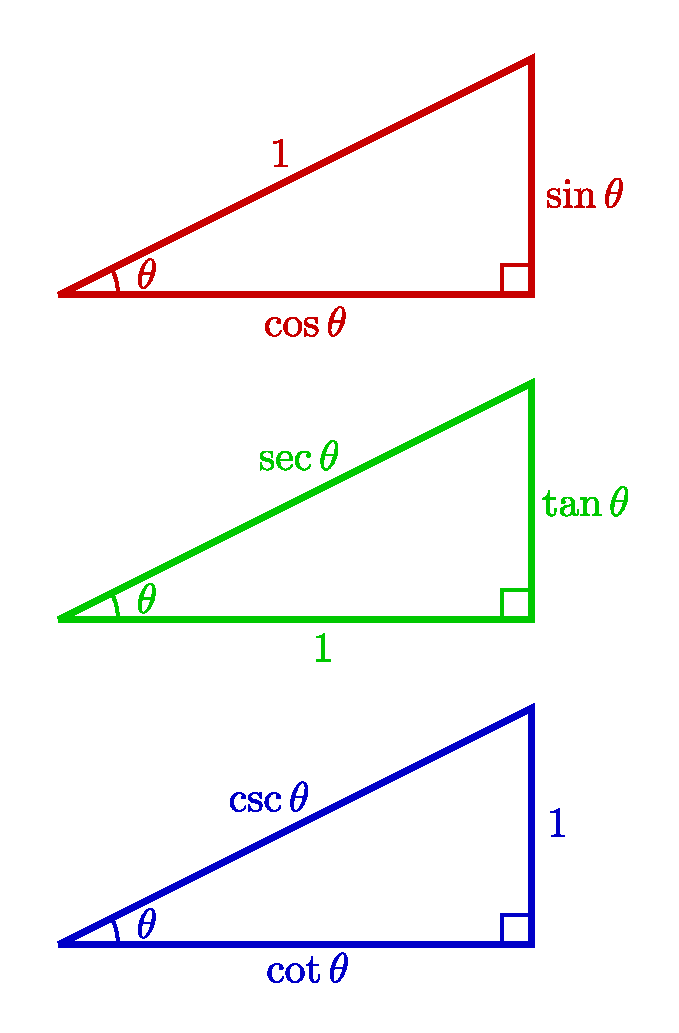
\includegraphics[width = 0.4\textwidth]{3_triangles}
}
\end{tabular}

Pythagorean Identities:
\begin{itemize}
\item \dr{\(\cos^2\theta + \sin^2\theta = 1\)}
\item \dg{\(\tan^2\theta + 1 = \sec^2\theta\)}
\item \db{\(\cot^2\theta + 1 = \csc^2\theta\)}
\end{itemize}

Replacing \(\theta\) with \(\theta + \pi\) gives:
\begin{itemize}
\item \dr{\(\cos(\theta + \pi) = -\cos\theta\)}
\item \dr{\(\sin(\theta + \pi) = -\sin\theta\)}
\item \dg{\(\tan(\theta + \pi) = \frac{\sin(\theta + \pi)}{\cos(\theta + \pi)} = \frac{-\sin\theta}{-\cos\theta} = \tan\theta\)}
\item \dg{\(\sec(\theta + \pi) = \frac{1}{\cos(\theta + \pi)} = \frac{1}{-\cos\theta} = -\sec\theta\)}
\item \db{\(\cot(\theta + \pi) = \frac{\cos(\theta + \pi)}{\sin(\theta + \pi)} = \frac{-\cos\theta}{-\sin\theta} = \cot\theta\)}
\item \db{\(\csc(\theta + \pi) = \frac{1}{\sin(\theta + \pi)} = \frac{1}{-\sin\theta} = -\csc\theta\)}
\end{itemize}

Replacing \(\theta\) with \(-\theta\) gives:
\begin{itemize}
\item \dr{\(\cos(-\theta) = \cos\theta\)}
\item \dr{\(\sin(-\theta) = -\sin\theta\)}
\item \dg{\(\tan(-\theta) = \frac{\sin(-\theta)}{\cos(-\theta)} = \frac{-\sin\theta}{\cos\theta} = -\tan\theta\)}
\item \dg{\(\sec(-\theta) = \frac{1}{\cos(-\theta)} = \frac{1}{\cos\theta} = \sec\theta\)}
\item \db{\(\cot(-\theta) = \frac{\cos(-\theta)}{\sin(-\theta)} = \frac{\cos\theta}{-\sin\theta} = -\cot\theta\)}
\item \db{\(\csc(-\theta) = \frac{1}{\sin(-\theta)} = \frac{1}{-\sin\theta} = -\csc\theta\)}
\end{itemize}

Replacing \(\theta\) with \(\pi/2-\theta\) gives:
\begin{itemize}
\item \dr{\(\cos(\pi/2-\theta) = \sin\theta\)}
\item \dr{\(\sin(\pi/2-\theta) = \cos\theta\)}
\item \dg{\(\tan(\pi/2-\theta) = \frac{\sin(\pi/2-\theta)}{\cos(\pi/2-\theta)} = \frac{\cos\theta}{\sin\theta} = \cot\theta\)}
\item \dg{\(\sec(\pi/2-\theta) = \frac{1}{\cos(\pi/2-\theta)} = \frac{1}{\sin\theta} = \csc\theta\)}
\item \db{\(\cot(\pi/2-\theta) = \frac{\cos(\pi/2-\theta)}{\sin(\pi/2-\theta)} = \frac{\sin\theta}{\cos\theta} = \tan\theta\)}
\item \db{\(\csc(\pi/2-\theta) = \frac{1}{\sin(\pi/2-\theta)} = \frac{1}{\cos\theta} = \sec\theta\)}
\end{itemize}


\end{document}










